In this section, we introduce the pricing framework that we are considering in this work. We start  by giving some details for the rBergomi model proposed in \cite{bayer2016pricing}. We then derive the formula of the price of a European call option under the rBergomi model in Section \ref{sec:Option pricing under rBergomi model}. Finally, we explain  some details about the schemes that we use to simulate the dynamics of asset prices under the rBergomi model.

\subsection{The rBergomi model}\label{sec:The rBergomi model}

We consider the rBergomi model for the price process $S_t$ as defined in  \cite{bayer2016pricing}, normalized to $r=0$\footnote{$r$ is the interest rate.}, which is defined by

\begin{align}\label{eq:rBergomi_model1}
	dS_t &= \sqrt{v_t} S_t dZ_t, \nonumber \\
	v_t &= \xi_0(t) \exp\left( \eta \widetilde{W}_t^H - \frac{1}{2} \eta^2 t^{2H} \right),
\end{align}
where the Hurst parameter $0 < H < 1$  and  $\eta>0$. We refer to $v_t$ as the variance process, and $\xi_0(t) = \expt{v_t}$ is  the forward variance curve.  Here, $\widetilde{W}^H $ is a certain Riemann-Liouville fBm
process\footnote{The so-called Riemann-Liouville processes are deduced from the standard Brownian motion by applying Riemann-Liouville fractional operators, whereas the standard fBm requires a weighted fractional operator \cite{marinucci1999alternative,picard2011representation}.},  defined by
\begin{align}\label{eq:Volterra process}
	\widetilde{W}_t^H = \int_0^t K^H(t,s) dW_s^1, \quad t \ge 0 \COMMA
\end{align}
where the kernel $K^H : \rset_+  \rightarrow \rset_+$ is
\begin{equation}\label{eq:kernel_rbergomi}
 \quad K^H(t-s) = \sqrt{2H} (t-s)^{H - 1/2},\quad \forall \: 0 \le s \le t.
\end{equation}
By construction, $\widetilde{W}^H $ is a centered, locally $(H-\epsilon)$- H\"older continuous, Gaussian process with $\text{Var}\left[\widetilde{W}^H_t \right] = t^{2H}$, and a dependence structure defined by 
 \begin{equation*}
 \expt{\widetilde{W}^H_u  \widetilde{W}^H_v}=u^{2H} G\left(\frac{v}{u} \right),\quad v >u \COMMA
 \end{equation*}
 where for $x \ge 1$ and $\gamma=\frac{1}{2}-H$
 \begin{equation}\label{eq:correlation_tilde_W_fun}
G(x)=2H \int_{0}^1 \frac{ds}{(1-s)^{\gamma} (x-s)^{\gamma}}.
 \end{equation}
%\red{We note that $\widetilde{W}$ is also a Brownian semi-stationary (BSS) process (see Definition \ref{def:semi-stationary process}), which was introduced by Barndorff-Nielsen and Schmiegel \cite{barndorff2007ambit,barndorff2009brownian}.
%
%\begin{definition}[Semi-stationary process]\label{def:semi-stationary process}
%$X_t$ is called a \textit{Brownian semi-stationary} process if
%\begin{equation}\label{eq:BSS}
%X_t=\int_{-\infty}^t K(t-s) \sigma_s dW_s\COMMA
%\end{equation}
%for some deterministic kernel function $K$ and an adapted intermittency process $\sigma$. If the integral starts at $0$ instead of $−\infty$
%\begin{equation}\label{eq:TBSS}
%X_t=\int_{0}^t K(t-s) \sigma_s dW_s\COMMA
%\end{equation}
%we call the process \textit{truncated Brownian semi-stationary} process (TBSS).
%\end{definition} 
%} 
In \eqref{eq:rBergomi_model1} and \eqref{eq:Volterra process}, $W^1, Z$ denote two \emph{correlated} standard Brownian motions with correlation $\rho \in ]-1,0]$, so that we can represent $Z$ in terms of $W^1$ as
\begin{align*}
	Z=\rho	W^1+ \bar{\rho}W^\perp = \rho W^1+\sqrt{1-\rho^2} W^\perp,
\end{align*}
where $(W^1,W^\perp)$ are two independent standard Brownian motions.
Therefore, the solution to \eqref{eq:rBergomi_model1}, with $S(0)=S_0$, can be written as 

\begin{align}\label{eq:rBergomi_model}
	S_t&= S_0  \operatorname{exp}\left( \int_{0}^{t} \sqrt{v(s)} dZ(s)- \frac{1}{2} \int_{0}^{t} v(s) ds   \right),\quad S_0>0 \nonumber\\
	v_u&=\xi_0(u) \operatorname{exp}\left( \eta \widetilde{W}_u^H- \frac{\eta^2}{2} u^{2H} \right), \quad \xi_0>0 \PERIOD
\end{align}
The filtration $(\mathcal{F}_t)_{t\ge 0}$ can here be taken as the one generated by the two-dimensional Brownian motion $(W^1,W^\perp)$ under the risk neutral measure $\mathbb{Q}$, resulting in  a filtered probability space $(\Omega,\mathcal{F}, \mathcal{F}_t,\mathbb{Q})$. The stock price process $S$ is clearly then a local
$(\mathcal{F}_t)_{t\ge 0}$-martingale and a supermartingale.  We shall henceforth use the notation $\expt{.} = E^{\mathbb{Q}}\left[. \mid \mathcal{F}_0\right]$ unless we state otherwise.
\begin{remark}
The rBergomi model is non-Markovian in the instantaneous variance $v_t$, that is $E^{\mathbb{Q}}\left[v_u\mid \mathcal{F}_t\right] \neq= E^{\mathbb{Q}}\left[v_u\mid v_t\right]$. However, it is Markovian in the state vector by definition, that is $E^{\mathbb{Q}}\left[v_u\mid\mathcal{F}_t\right]=\xi_t(u)$.
\end{remark}
\subsection{Option pricing under the rBergomi model}\label{sec:Option pricing under rBergomi model}

We are interested in pricing European call options under the rBergomi model. Assuming $S_0 = 1$, and using the conditioning argument on the $\sigma$-algebra generated by $W^1$ (an argument first used by \cite{romano1997contingent} in the context of Markovian stochastic volatility  models), we can  show that the call price is given by

\begin{align}\label{BS_formula_rbergomi}
	C_{\text{RB}}\left( T, K \right) &= \text{E}\left[ \left(S_T - K \right)^+ \right]  \nonumber\\
	&=\expt{\expt{(S_T-K)^+ \mid \sigma(W^1(t) ,t \le T)}}\nonumber \\
	&=\text{E}\left[C_{\text{BS}}\left( S_0 = \operatorname{exp}\left(\rho \int_0^T \sqrt{v_t} dW_t^1 - \frac{1}{2}
	\rho^2 \int_0^T v_t dt\right),\ k = K, \ \sigma^2 = (1-\rho^2)
	\int_0^T v_t dt \right) \right],
\end{align}
where $C_{\text{BS}}(S_0,k,\sigma^2)$ denotes the Black-Scholes call price, for initial spot price $S_0$, strike price $k$ and volatility $\sigma^2$.

%To show \eqref{BS_formula_rbergomi}, we use the orthogonal decomposition of $S_t$ into $S_{t}^1$ and $S_{t}^2$, where
%\begin{align*}
%	S_t^1=\mathcal{E}\{ \rho \int_{0}^{t}  \sqrt{v_s} dW_s^1\}, \: S_t^2= \mathcal{E}\{ \sqrt{1-\rho^2} \int_{0}^{t}  \sqrt{v_s} dW_s^\perp  \}	,
%\end{align*}
%and $\mathcal{E}(.)$ denotes the stochastic exponential; then, if we define $\mathcal{F}_t^1= \sigma\{ W_s^1: s\le t\}$, we obtain by conditional log-normality
%\begin{align*}
%	\log S_t \mid \mathcal{F}_t^1 \sim \mathcal{N}\left( \log S_t^1-\frac{1}{2} (1-\rho^2) \int_{0}^{t} v_s ds , (1-\rho^2) \int_{0}^{t} v_s ds \right),
%\end{align*} 
%and by using the same procedure as in \cite{romano1997contingent} we obtain \eqref{BS_formula_rbergomi}.

We point out that the analytical smoothing, based on conditioning, performed in \eqref{BS_formula_rbergomi} enables us to uncover the available regularity, and hence  get a smooth, analytic integrand inside the expectation. Therefore, applying a deterministic quadrature technique such as ASGQ or QMC becomes an adequate option for computing the call price as we will investigate later. A similar conditioning was used in \cite{mccrickerd2018turbocharging} but for variance reduction purposes only.

\subsection{Simulation of the rBergomi model}\label{sec:Simulation of the rBergomi model}

One of the numerical challenges encountered in the simulation of the rBergomi dynamics  is the computation of  $\int_{0}^{T} \sqrt{v_t} dW_t^1$ and $V=\int_{0}^{T} v_t dt$ in \eqref{BS_formula_rbergomi}, mainly because of the singularity of the Volterra kernel $K^H(s,t)$ at the diagonal $s = t$. In fact,  one needs to jointly simulate two Gaussian processes $(W_t^1, \widetilde{W}^H_t: 0 \le t \le T)$, resulting in $W^1_{t_1},\dots, W^1_{t_N}$ and $\widetilde{W}^H_{t_1},\dots, \widetilde{W}^H_{t_N}$ along a given time grid $t_1 <\dots < t_N$. In the literature, there are essentially two suggested ways to achieve this:
 \begin{enumerate}
% 	\item[i)] \textbf{Simple Euler discretization}: Euler discretization of the integral \eqref{eq:Volterra process}, defining $\widetilde{W}^H$, together with classical simulation of increments of $W^1$. This is inefficient because the integral is singular and adaptivity may not improve the scheme since the singularity moves with time. For this method, we need an $N$-dimensional random Gaussian input vector to produce one (approximate, inaccurate) sample of $W^1_{t_1},\dots, W^1_{t_N}, \widetilde{W}^H_{t_1},\dots, \widetilde{W}_{t_N}$.
 	
 	\item[i)] \textbf{Covariance based approach (exact simulation) \cite{bayer2016pricing,bayer2018short}}: $W^1_{t_1},\dots, W^1_{t_N}, \widetilde{W}^H_{t_1},\dots, \widetilde{W}_{t_N}$ together form a ($2N$)-dimensional Gaussian random vector with computable covariance matrix, and therefore one can use Cholesky decomposition of the covariance matrix to produce exact samples of $W^1_{t_1},\dots, W^1_{t_N}, \widetilde{W}^H_{t_1},\dots, \widetilde{W}_{t_N}$ from $2 N$-dimensional Gaussian random vector as  input. This method is exact but slow. The simulation  requires $\Ordo{N^2}$ flops. Note that the offline cost is $\Ordo{N^3}$ flops.
 	
 	\item[ii)]  \textbf{The hybrid scheme of \cite{bennedsen2017hybrid}}: This scheme uses a different approach, which is essentially based on  Euler discretization  but crucially improved by moment
 	matching for the singular term in the left point rule. It is also
 	inexact in the sense that samples produced here do not exactly have the distribution of $W^1_{t_1},\dots, W^1_{t_N}, \widetilde{W}^H_{t_1},\dots, \widetilde{W}_{t_N}$, however they are much more accurate than samples produced from simple Euler discretization, but much faster than method $(i)$. As in method $(i)$, in this case, we need a $2 N$-dimensional Gaussian random input vector to produce one 	sample of $W^1_{t_1},\dots, W^1_{t_N}, \widetilde{W}^H_{t_1},\dots, \widetilde{W}_{t_N}$.
 \end{enumerate} 

\subsubsection{On the choice of the simulation scheme in our approach}\label{sec: choice of simulation scheme}
The choice of the simulation scheme in our approach was based on the observed behavior of the weak rates. Through our numerical experiments (see Table \ref{table:Reference solution, using MC with $500$ time steps, of Call option price under rBergomi model, for different parameter constellation.} for the tested examples), we observe that although the hybrid and exact schemes  converge asymptotically with weak rate of $\Ordo{\Delta t}$, the pre-asymptotic behavior of the weak rate is different for both schemes. As an illustration, from Figure \ref{fig:Weak_rate_set1_set_2_without_rich_hyb+chol} for Set $1$ parameter in Table \ref{table:Reference solution, using MC with $500$ time steps, of Call option price under rBergomi model, for different parameter constellation.}, the hybrid scheme  has a consistent convergence behavior in the sense that it behaves in the asymptotic way basically right from the beginning, whereas the exact scheme does not. On the other
hand, the constant  seems considerably smaller for the exact scheme. These two features  make the hybrid scheme the optimal scheme  to work with in our context since our approach is based on hierarchical transformations involving the use of Richardson extrapolation (see Section \ref{sec:Richardson extrapolation}).
\FloatBarrier
\begin{figure}[h!]
	\centering
	\begin{subfigure}{.4\textwidth}
		\centering
		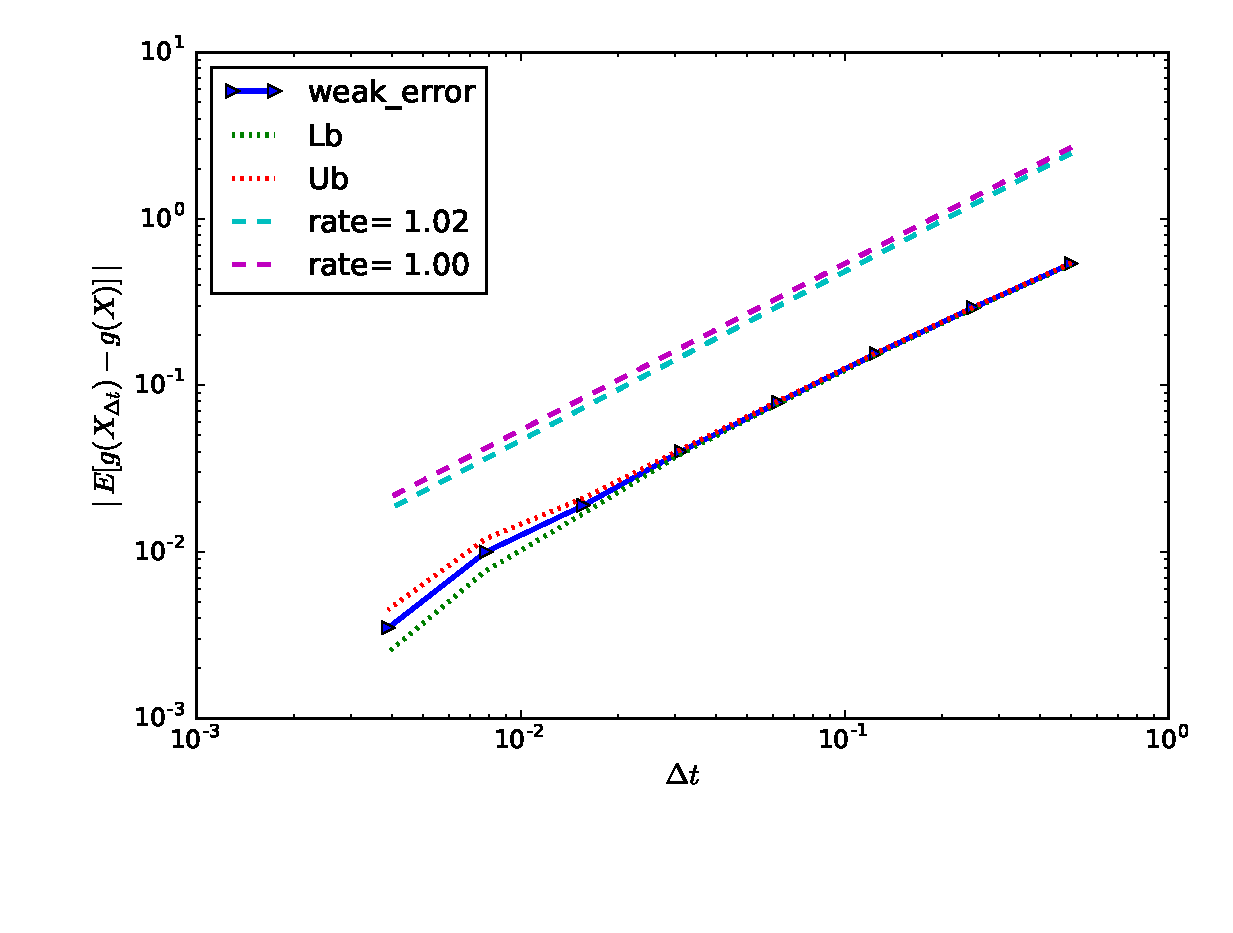
\includegraphics[width=1\linewidth]{./figures/rBergomi_weak_error_rates/without_richardson/H_007/weak_convergence_order_Bergomi_H_007_K_1_M_4_10_6_CI_relative_hybrid_non_hierarchical_non_parallel_asymptotic}
		\caption{}
		\label{fig:set1_weak_rate_hybrid}
	\end{subfigure}%
	\begin{subfigure}{.4\textwidth}
		\centering
		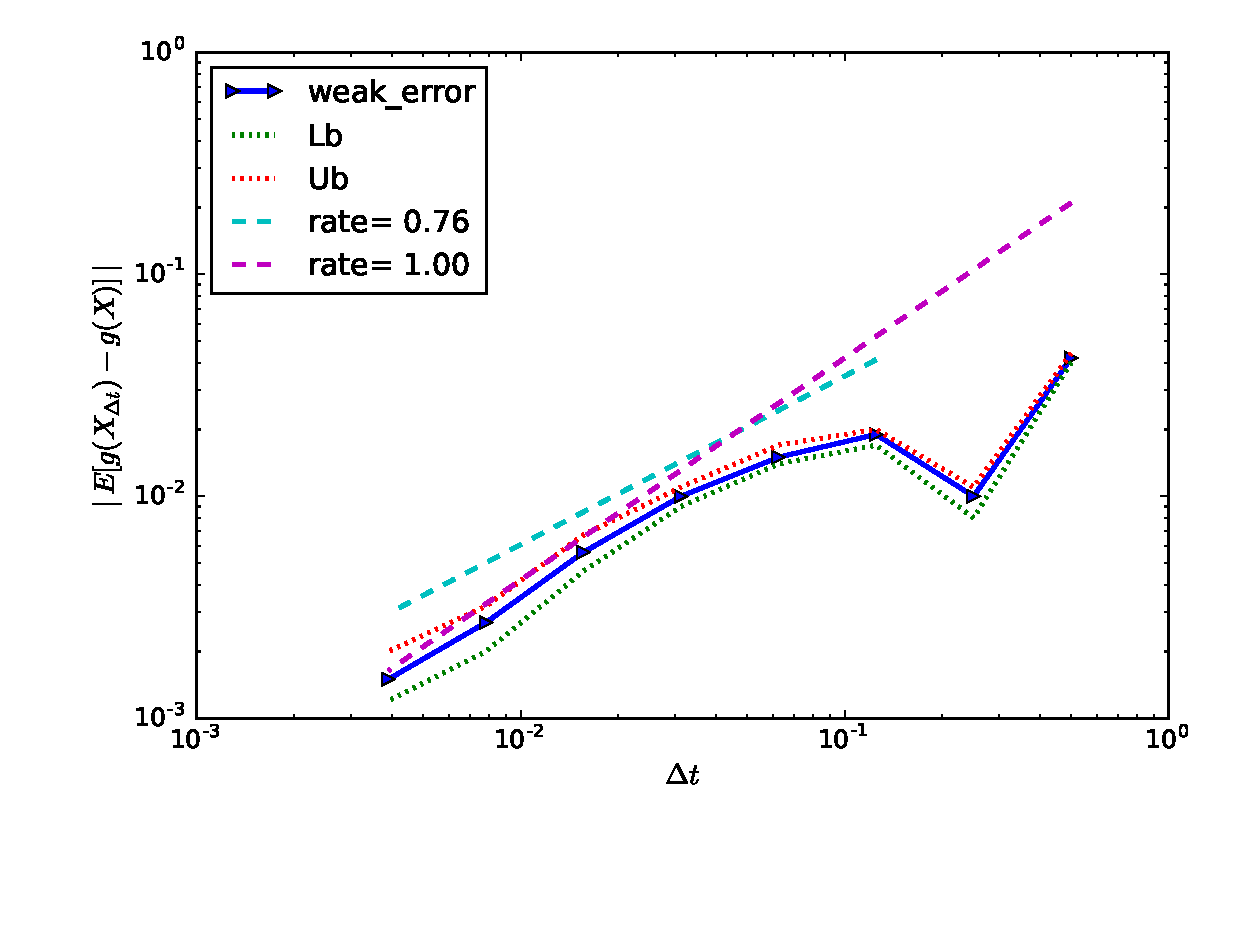
\includegraphics[width=1\linewidth]{./figures/rBergomi_weak_error_cholesky/weak_convergence_order_Bergomi_H_007_K_1_M_4_10_6_CI_relative_cholesky_non_hierarchical_non_parallel_asymptotic}
		\caption{}
		\label{fig:set1_weak_rate_exact}
	\end{subfigure}
	\caption{The convergence of the weak error $\mathcal{E}_B$, using MC with $6 \times 10^6$ samples, for Set $1$ parameter in Table \ref{table:Reference solution, using MC with $500$ time steps, of Call option price under rBergomi model, for different parameter constellation.}. We refer to $C_{\text{RB}}$ (as in \eqref{BS_formula_rbergomi}) for $\expt{g(X)}$, and to $C_{\text{RB}}^{N}$ (as in \eqref{BS_formula_rbergomi_2}) for $\expt{g(X_{\Delta t})}$. The upper and lower bounds are $95\%$ confidence intervals. a) With the hybrid scheme  b) With the exact scheme.}
	\label{fig:Weak_rate_set1_set_2_without_rich_hyb+chol}
\end{figure}
\FloatBarrier

\subsubsection{The hybrid scheme}\label{sec: The hybrid scheme}
As motivated in Section  \ref{sec: choice of simulation scheme}, in this work, we use the hybrid scheme which,  on equidistant grid $\{0,\frac{1}{N},\frac{2}{N},\dots,\frac{NT}{N}\}$, is given by 
the following,
\begin{align}\label{eq:Hybrid_scheme_pre}
\widetilde{W}^H_{\frac{i}{N}} \approx \bar{W}^H_{\frac{i}{N}}&= \sqrt{2H} \left(  \sum_{k=1}^{\min(i,\kappa)} \int_{\frac{i}{N}-\frac{k}{N}}^{\frac{i}{N}-\frac{k}{N}+\frac{1}{N}} \left(\frac{i}{N}-s\right)^{H - 1/2} dW^1_s+\sum_{k=\kappa+1}^{i} \left(\frac{b_k}{N}\right)^{H - 1/2}  \int_{\frac{i}{N}-\frac{k}{N}}^{\frac{i}{N}-\frac{k}{N}+\frac{1}{N}} dW^1_s \right) \COMMA
\end{align}
which results for $\kappa=1$  in \eqref{eq:Hybrid_scheme}.
\begin{align}\label{eq:Hybrid_scheme}
\widetilde{W}^H_{\frac{i}{N}} \approx \bar{W}^H_{\frac{i}{N}}&= \sqrt{2H} \left(  W^2_i+\sum_{k=2}^{i} \left(\frac{b_k}{N}\right)^{H-\frac{1}{2}} \left(W_{\frac{i-(k-1)}{N}}^1-W_{\frac{i-k}{N}}^1\right)\right)\COMMA
\end{align}
where $N$ is the number of time steps and 
$$ b_k=\left(\frac{k^{H+\frac{1}{2}}-(k-1)^{H+\frac{1}{2} }}{H+\frac{1}{2}}\right)^{\frac{1}{H-\frac{1}{2}}} \PERIOD$$
The sum in \eqref{eq:Hybrid_scheme} requires the most computational effort in the simulation. Given that \eqref{eq:Hybrid_scheme} can be seen as discrete convolution  (see \cite{bennedsen2017hybrid}), we employ the fast Fourier transform to evaluate it, which results in  $\Ordo{N \log N}$ floating point operations.

We note that the variates $\bar{W}_0^{H},\bar{W}_1^{H},\dots,\bar{W}_{\frac{[Nt]}{N}}^{H}$ are  generated by sampling $[Nt]$ i.i.d draws from a $(\kappa+1)$-dimensional Gaussian distribution and computing a discrete convolution. We denote these pairs  of Gaussian random variables from now on by $(\mathbf{W}^{(1)},\mathbf{W}^{(2)})$. 
%\red{In the following, we give more details for each scheme.}
%\red{\subsubsection{The exact scheme}\label{sec:The Exact Scheme}
%The exact scheme is based on simulating exactly the joint covariance of $(\widetilde{W}^H,W^1)$, which is given by
%\begin{align}\label{eq:joint covariance cholesky}
% \begin{cases}
%               \text{Var}(\widetilde{W}_t)=t^{2H}&,\quad t \ge 0\\
%                \text{Cov}(\widetilde{W}_t,\widetilde{W}_s)=t^{2H} G\left(\frac{s}{t}\right)&,\quad s>t \ge 0\\
%              \text{Cov}(\widetilde{W}_t,W^1_s)=\rho D_H \left(t^{H+\frac{1}{2}}-\left( t-\min(t,s)^{H+\frac{1}{2}} \right) \right) &,\quad s,t \ge 0\\
%              \text{Cov}(W^1_t,W^1_s)=\min(t,s)&,\quad s,t \ge 0\COMMA
%            \end{cases}
%\end{align}
%with 
%$$ D_H=\frac{\sqrt{2H}}{H+\frac{1}{2}}$$
%and $G$ is given by \eqref{eq:correlation_tilde_W_fun} for $x \ge 1$ and $\gamma=\frac{1}{2}-H$.
%%Different ways can be used to compute  \eqref{eq:correlation_tilde_W_fun}. For instance, in the literature we find that  in \cite{bayer2018short}
%%\begin{equation}
%%G_2(x)=2H \left(  \frac{1}{1-\gamma} x^{-\gamma}+\frac{\gamma}{1-\gamma}x^{-(1+\gamma)} \frac{1}{2-\gamma} {}_2F_1\left(1,1+\gamma,3-\gamma,x^{-1} \right)  \right),
%%\end{equation}
%%where 
%%\begin{align*}
%%{}_2F_1(a,b,c;z)=\frac{\Gamma(c)}{\Gamma(b) \Gamma(c-b)} \int_{0}^1 t^{b-1} (1-t)^{c-b-1} (1-tz)^{-a} dt.
%%\end{align*}
%\begin{remark}
%Since the covariance matrix does not have any $0$ values, if $\rho\neq0$, the computational effort for the exact simulation is quite high and the algorithm is very slow.
%\end{remark}
%}
%\red{
%\subsubsection{The hybrid scheme}
%The hybrid scheme was developed in \cite{bennedsen2017hybrid} for the simulation of BSS \eqref{eq:BSS} and TBSS \eqref{eq:TBSS} processes with kernel functions, that are similar to a power function near zero, i.e. $K(x)$ is similar to $x^\alpha$ for some $\alpha \in(-\frac{1}{2},\frac{1}{2})$ when $x>0$ is near zero. 
%
%In this section, we start by introducing the general idea of the hybrid scheme. Then, we illustrate how it can be used in simulating  rBergomi  dynamics.
%\subsubsection*{General idea of the hybrid scheme}
%Before describing the general hybrid scheme, there are two assumptions (conditions) that should be fulfilled by the kernel function $K$ in order to apply the scheme. In fact, we assume that the kernel function $K:(0,\infty)\rightarrow [0,\infty)$ satisfy the following
%\begin{enumerate}
%\item For some $\alpha \in(-\frac{1}{2},\frac{1}{2})\setminus\{0\}$,
%$$ K(x)=x^\alpha L_K(x),\quad x \in (0,1],$$
%where $L_K:(0,1] \rightarrow [0,\infty)$ is continuously differentiable, slowly varying at $0$ and bounded away from $0$. Moreover there exists a constant $C>0$ such that the derivative $L^\prime_K$ satisfies
%$$ \abs{L_K^\prime(x)} \le C \left(1+x^{-1}\right),\quad x \in (0,1].$$
%\item The function $K$ is continuously differentiable on $(0,\infty)$, with derivative $K^\prime$ that is ultimately monotonic and also satisfies $\int_{1}^ \infty K^\prime(x)^2 dx<\infty$.
%\end{enumerate}
%The hybrid scheme starts by discretizing a TBSS process $X_t$ giving by \eqref{eq:TBSS} on the grid $G_{t}^N=\{t,t-\frac{1}{N},t-\frac{2}{N},\dots\}$ for $N \in \nset^{+}$, so that we get
%\begin{align}\label{eq:hybrid_scheme_1}
%X_t \approx \sum_{k=1}^{N_N} \sigma_{t-\frac{k}{N}} \int_{t-\frac{k}{N}}^{t-\frac{k}{N}+\frac{1}{N}} K(t-s)  dW_s,
%\end{align}
% where $N_N \in \nset^+$ is the truncation parameter and $N$ denotes the number of discretization steps, and we assume that $\sigma$ does not vary too much (valid in the rBergomi model since $\sigma$ is constant), therefore constant in each discretization cell.
% 
%The idea of the hybrid scheme  is to split the kernel function into two parts \eqref{eq:kernel approximation_hybrid}, depending on a small parameter $\kappa$\footnote{There are different variants of the hybrid scheme depending on the value of $\kappa$ (see \cite{bennedsen2017hybrid} for more details).} 
%\begin{align}\label{eq:kernel approximation_hybrid}
% K(t-s)\approx\begin{cases}
%              (t-s)^\alpha L_K\left(\frac{k}{N}\right), \quad t-s \in \left[\frac{k-1}{N},\frac{k}{N}\right] \setminus \{0\}&, \quad \text{if} \: k \le \kappa \\
%           K\left(\frac{b_k}{N}\right) , \quad t-s \in \left[\frac{k-1}{N},\frac{k}{N}\right] &, \quad \text{if}\:  k >\kappa,
%            \end{cases}
%\end{align}
%and then discretizing the  $X_t$ process into Wiener integrals of power functions and a Riemann sum, appearing from approximating the kernel by power functions near the origin and step functions elsewhere, resulting in \eqref{eq:hybrid_scheme_2}
%\begin{align}\label{eq:hybrid_scheme_2}
%X_t \approx \sum_{k=1}^\kappa    L_K\left(\frac{k}{N}\right) \sigma_{t-\frac{k}{N}} \int_{t-\frac{k}{N}}^{t-\frac{k}{N}+\frac{1}{N}} (t-s)^\alpha   dW_s+ \sum_{k=\kappa+1}^{N_N}   K\left(\frac{b_k}{N}\right) \sigma_{t-\frac{k}{N}} \int_{t-\frac{k}{N}}^{t-\frac{k}{N}+\frac{1}{N}}   dW_s \PERIOD
%\end{align}
%\begin{remark}
%$\left(b_k\right)_{k=\kappa+1}^\infty$ is a sequence of real numbers that only needs to satisfy  $b_k \in \left[k-1, k\right]\setminus \{0\}$. But there is an optimal sequence $\left(b_k^\ast\right)_{k=\kappa+1}^\infty$, that minimizes the asymptotic \textit{mean square error} (see \cite{bennedsen2017hybrid} for more details) and it is given by
%$$ b_k^\ast=\left(\frac{k^{\alpha+1}-(k-1)^{\alpha+1 }}{\alpha+1}\right)^{\frac{1}{\alpha}},\quad k \ge \kappa+1 \PERIOD$$
%\end{remark}

%\subsubsection*{The hybrid scheme in the rBergomi context}
%In the context of the rBergomi model, we have $\sigma=1$, $\alpha=H-\frac{1}{2}$ and we can  use the hybrid scheme to simulate $\widetilde{W}^H_t$, which is  a TBSS process, with the kernel function $K^H$ given by \eqref{eq:kernel_rbergomi}. In this context, we can show that by choosing $L_{K^H}(x)=1$, we have  $K^H$ satisfy the conditions required to apply the hybrid scheme  (see \cite{bennedsen2017hybrid}) and therefore we end up with
%the following scheme on equidistant grid $\{0,\frac{1}{N},\frac{2}{N},\dots,\frac{NT}{N}\}$
%\begin{align}\label{eq:Hybrid_scheme_pre}
%\widetilde{W}^H_{\frac{i}{N}} \approx \bar{W}^H_{\frac{i}{N}}&= \sqrt{2H} \left(  \sum_{k=1}^{\min(i,\kappa)} \int_{\frac{i}{N}-\frac{k}{N}}^{\frac{i}{N}-\frac{k}{N}+\frac{1}{N}} \left(\frac{i}{N}-s\right)^{H - 1/2} dW^1_s+\sum_{k=\kappa+1}^{i} \left(\frac{b_k}{N}\right)^{H - 1/2}  \int_{\frac{i}{N}-\frac{k}{N}}^{\frac{i}{N}-\frac{k}{N}+\frac{1}{N}} dW^1_s \right) \COMMA
%\end{align}
%which results for $\kappa=1$  in \eqref{eq:Hybrid_scheme}.
%\begin{align}\label{eq:Hybrid_scheme}
%\widetilde{W}^H_{\frac{i}{N}} \approx \bar{W}^H_{\frac{i}{N}}&= \sqrt{2H} \left(  W^2_i+\sum_{k=2}^{i} \left(\frac{b_k}{N}\right)^{H-\frac{1}{2}} \left(W_{\frac{i-(k-1)}{N}}^1-W_{\frac{i-k}{N}}^1\right)\right)\COMMA
%\end{align}
%where $N$ is the number of time steps and 
%$$ b_k=\left(\frac{k^{H+\frac{1}{2}}-(k-1)^{H+\frac{1}{2} }}{H+\frac{1}{2}}\right)^{\frac{1}{H-\frac{1}{2}}} \PERIOD$$
%The sum in \eqref{eq:Hybrid_scheme} requires the most computational effort in the simulation. Given that \eqref{eq:Hybrid_scheme} can be seen as discrete convolution  (see \cite{bennedsen2017hybrid}), we employ the fast Fourier transform to evaluate it, which results in  $\Ordo{N \log N}$ floating point operations.
%
%We note that the variates $\bar{W}_0^{H},\bar{W}_1^{H},\dots,\bar{W}_{\frac{[Nt]}{N}}^{H}$ are  generated by sampling $[Nt]$ i.i.d draws from a $(\kappa+1)$-dimensional Gaussian distribution and computing a discrete convolution. We denote these pairs  of Gaussian random variables from now on by $(\mathbf{W}^{(1)},\mathbf{W}^{(2)})$.
%}
%

